\documentclass[unicode,bookmarksnumbered]{beamer}

\usepackage{lmodern} % Sázet se bude Latin Modern fonty, nikoli výchozími EC fonty.
\usepackage[czech, english]{babel}
\usepackage[utf8]{inputenc}
\usepackage[T1]{fontenc}
%\usepackage{cmap}

\usepackage{graphicx}
\usepackage{color}
\usepackage{hyperref} 

%\usepackage{times}

\usetheme{Warsaw}%Berlin
\usecolortheme{beaver}%dolphin}

% \setbeamercovered{invisible}		%zadne - nejsou videt
% \setbeamercovered{transparent}	%jsou videt / ale jen trochu
\setbeamercovered{dynamic}		%prvni volba zvyraznena, dalsi dve tranparentni, postupne se zvyraznuji dalsi
% \setbeamercovered{highly dynamic}	%zvyrazneni neaktivnich casti seznamu 

% nasledujici volba zpusobi, ze vycty v~prezentaci se zobrazuji postupne
%\beamerdefaultoverlayspecification{<+->}

\usepackage{multimedia}

\title[Zásuvný modul QGIS pro slučování vektorových map]{Bakalářská práce}
\subtitle{Zásuvný modul QGIS pro slučování vektorových map}
\author{Tereza Fiedlerová} 

\institute[ČVUT]{ČESKÉ VYSOKÉ UČENÍ TECHNICKÉ V PRAZE\\
		Katedra mapování a~kartografie}

\def\denD{25.\,6.\,2013} % den prezentace
\date[červen 2013]{{\denD} / obhajoba }

\logo{\includegraphics[scale=0.4]{./pictures/logo.pdf} }

\setbeamercolor{block title}{bg=red!40!black,fg=white}  % nastavení barvy definic apod.
%\setbeamercolor{block body}{bg=white,fg=black}
\setbeamercolor*{item}{fg=red!60!black}  % nastavení barvy puntíků

%zacatek dokumentu
\begin{document}

  \begin{frame}
    \titlepage % uvodni stranka
  \end{frame}

%   \begin{frame}  % uvést o čem budu mluvit
%     \frametitle{Obsah}
%     \setcounter{tocdepth}{1}
%     \tableofcontents 
%   \end{frame}

  \section{Zadání}  % říct zadání a~cíle práce
  \begin{frame}
   \frametitle{Zadání}
    Hlavní cíl:
     \begin{itemize}
      \item nastudování problematiky slučování vektorových dat
     \end{itemize}
     Dle oficiálního zadání:
     \begin{itemize}
      \item návrh a~implementace zásuvného modulu pro QGIS
      \item návrh C++ knihovny obsahující vybrané algoritmy
      \item přehled existujících nástrojů umožňujících slučování map
     \end{itemize}
  \end{frame}

\section{Conflation}  % spíše stručně vysvětlit co to je, dělení, kdy to vzniklo ...

  \subsection{Pojem conflation}
  \begin{frame}
  \frametitle{Pojem \textit{conflation}}

    \begin{block}{Encyklopedická definice}
     Proces kombinování geografických informací z překrývajících se
     zdrojových dat, který zachovává přesnost dat, minimalizuje 
     nadbytečná data a~předchází konfliktům v~datech.
    \end{block}
     {\small(Shekhar, Xiong: Encyclopedia of GIS)}

    \begin{block}{Stručná definice}
     Proces sjednocení dvou rozdílných datových sad.
    \end{block}
     {\small(Blasby a~kol.: GIS Conflation Using Open Source Tools)}

  \end{frame}

%   \subsection{Klasifikace} % šla by zmínit ve slidu s definicí
%   \begin{frame}
%   \frametitle{Klasifikace} % obrázek?
%     \textbf{Dle typu vstupních vrstev:}
%      \begin{itemize}
%       \item rastr - rastr (imagery to imagery)
%       \item rastr - vektor (vector to imagery)
%       \item \textcolor{red!70!black}{vektor - vektor} (vector to vector)
%      \end{itemize}
%     \textbf{Dle území zobrazovaného vstupními vrstvami:}
%      \begin{itemize}
%       \item horizontální
%         \begin{itemize}
%          \item vrstvy zobrazující sousedící území
%         \end{itemize}
%       \item vertikální
%         \begin{itemize}
%          \item vrstvy zobrazující překrývající se území
%         \end{itemize}
%      \end{itemize}
%   \end{frame}

  \subsection{Obecný postup}
  \begin{frame}
  \frametitle{Obecný postup}   % stručně popsat, první dva kroky a~poslední krok bývá v~režii uživatele, zbytek by měl vykonat conflation systém
     \textbf{Postup při slučování vektorových dat:}
     \begin{enumerate}
      \item Předzpracování dat% (zajištění kompatibility)
      \item Kontrola kvality dat a~topologické správnosti vrstev
      \item Vyhledání odpovídajících si prvků
      \item Sloučení geometrických prvků a/nebo jejich atributů
      \item Závěrečné úpravy %(kontrola, drobné opravy)
     \end{enumerate}
      \pause[]
     Úkolem programu pro automatické sloučení dat jsou kroky 3 a~4,
     zbytek je ponechán většinou na uživateli.
  \end{frame}


\section{Existující nástroje} % vyjmenovat, podrobněji možná jen k ArcGIS a~JCS

  \subsection{Proprietární nástroje}
  \begin{frame}
    \frametitle{Proprietární nástroje}
     \begin{itemize}
      \item ESRI ArcGIS - Spatial Adjustment, Integrate
	  \begin{itemize}
	    \item dílčí nástroje umožňující různé operace
	  \end{itemize}
      \item Intergraph Geomedia - Fusion
	  \begin{itemize}
	    \item údržba dat v~geografických databázích, %topologické opravy, 
		  integrace dat
	  \end{itemize}
      \item ESEA MapMerger
	  \begin{itemize}
	    \item převod atributů, aktualizace a~kombinace dvou map
	  \end{itemize}
      \item ConfleX
	  \begin{itemize}
	    \item využití umělé inteligence%, porovnávání jednotlivých segmentů
		  %a~topologických vztahů
	  \end{itemize}
     \end{itemize}
  \end{frame}

  \subsection{Open Source nástroje}
  \begin{frame}
    \frametitle{Open Source nástroje}
	\begin{itemize}
	  \item JCS - Java Conflation Suite
	      \begin{itemize}
		\item jediný ucelenější nástroj v~této skupině
		\item knihovna založená na JTS (Java Topology Suite)
		\item kolekce zásuvných modulů pro OpenJUMP %- QA, Conflate, RoadMatcher
	      \end{itemize}
	  \item OpenStreetMap
	      \begin{itemize}
		%\item JOSM conflation, Potlatch2merging tool
		\item drobné nástroje, spíše ruční slučování map
	      \end{itemize}
	\end{itemize} 
  \end{frame}


\section{Knihovna GEOC}   % jak byla navržena, proč samostatná knihovna, stručný popis jednotlivých algoritmů + rovnou i problémy a~jejich řešení

  \subsection{GEOC}
  \begin{frame}
  \frametitle{GEOC}
     \begin{itemize}
      \item knihovna s~algoritmy pro slučování vektorových map
      \item navržena nezávisle na QGIS zásuvném modulu 
      \item využívá knihovnu GEOS (Geometry Engine, Open Source)
      \begin{itemize}
       \item přepis knihovny JTS do C++
       \item reprezentace geometrie
       \item prostorové vztahy a operace
      \end{itemize}

     \end{itemize}
  \end{frame}

  \subsection{Vertex Snapper}  % obrázek
  \begin{frame}
  \frametitle{Vertex Snapper}
    \framesubtitle{Přichycení vrcholů}
    \begin{columns}[c]
	\column{2in}
	\begin{enumerate}
	   \item určení vzdálenostní tolerance
	   \item nalezení blízkých prvků
	   \item výpočet vzdáleností mezi vrcholy blízkých prvků
	   \item přichycení dvou nejbližších vrcholů
	\end{enumerate}
	\column{2in}
	  \begin{figure}
	  \centering
             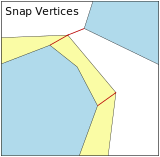
\includegraphics[width=1.5in]{./pictures/snap.pdf}
	  \label{fig:vs-princip}
	  \end{figure}
      \end{columns}
  \end{frame}

  \subsection{Coverage Alignment} % obrázek
  \begin{frame}
  \frametitle{Coverage Alignment}
    \framesubtitle{Zarovnání vrstev}
    \begin{columns}[c]
	\column{2in}
	\begin{enumerate}
	   \item nalezení odpovídajících si prvků
	   \item určení bodů pro TIN
	   \item Delaunayho triangulace 
	   \item lokální afinní transformace
	   \item případně další iterace
	\end{enumerate}
	\column{2in}
	  \begin{figure}
	  \centering
             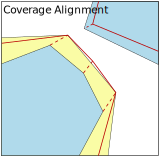
\includegraphics[width=1.5in]{./pictures/align.pdf}
	  \label{fig:ca-princip}
	  \end{figure}
      \end{columns}
  \end{frame}

  \begin{frame}
  \frametitle{Coverage Alignment}
    \framesubtitle{Nalezení odpovídajících si prvků}
    \footnotesize 
    \begin{columns}[c]
	\column{2in}
	Test obalových zón prvků
	\begin{figure}
	  \centering
	    \includegraphics[width=2.5in]{./pictures/buffer-test.pdf}
	  \label{fig:ca1}
	  \end{figure}
	\column{2in}
	Test obalových zón hranic prvků
	  \begin{figure}
	  \centering
	    \includegraphics[width=2.5in]{./pictures/buffer-boundary.pdf}
	  \label{fig:ca2}
	  \end{figure}
    \end{columns}
  \end{frame}

  \subsection{Line Matcher} % obrázek
  \begin{frame}
  \frametitle{Line Matcher}
    \framesubtitle{Spojování linií}
     \begin{columns}[c]
	\column{2in}
	\begin{enumerate}
	    \item nalezení blízkých linií% k~danému segmentu
	    \item testování segmentu s~každým úsekem blízké linie
	    \item určení nejpodobnějšího segmentu
		  (délka, úhel, blízkost) 
	    \item průměr z~podobných segmentů
	\end{enumerate}
	\column{2in}
	  \begin{figure}
	  \centering
             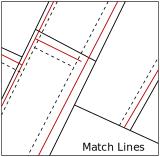
\includegraphics[width=1.5in]{./pictures/match.pdf}
	  \label{fig:lm-princip}
	  \end{figure}
      \end{columns}
  \end{frame}


\section{Zásuvný modul Conflate}   % obecně o pluginech pro QGIS, konkrétní návrh mého zásuvného modulu

  \subsection{Conflate} % obrázek
  \begin{frame}
  \frametitle{Conflate}
    \begin{columns}[c]
	\column{2.5in}
     \begin{itemize}
      \item zásuvný modul pro Quantum GIS
      \item psaný v~jazyce C++
      \item využití algoritmů knihovny GEOC
     \end{itemize}
     	\column{1.5in}
	  \begin{figure}
             
\includegraphics[width=0.6in]{./pictures/icon.pdf}
	  \label{fig:icon}
	  \end{figure}
      \end{columns}
    \vspace{0.5cm}
     \begin{figure}
      \centering
      \scriptsize
      \def\svgwidth{4in}
      \input{./pictures/schema.pdf_tex}
      \label{fig:schema}
  \end{figure} 
  \end{frame}

  \subsection{GUI} % až na závěr
  \begin{frame}
  \frametitle{Grafické uživatelské rozhraní}
     \begin{figure}
	  \centering
             \includegraphics[height=2.5in]{./pictures/dialog2.png}
	  \label{fig:dialog1}
	  \end{figure}
  \end{frame}

  \begin{frame}
  \frametitle{Grafické uživatelské rozhraní}
     \begin{figure}
	  \centering
             \includegraphics[height=2.5in]{./pictures/dialog4.png}
	  \label{fig:dialog2}
	  \end{figure}
  \end{frame}


  \begin{frame}
  \frametitle{Ukázka zarovnání vrstev}
     \begin{figure}
	  \centering
	  \scriptsize
	    \def\svgwidth{4in}
             \input{./pictures/test-ca-porovnani.pdf_tex}
	  \label{fig:ukazka}
	  \end{figure}
  \end{frame}

%   \subsection{Ukázka} % až na závěr
%   \begin{frame}
%   \frametitle{Ukázka}
%    \movie[autostart,externalviewer]{}{out.ogv}
%   \end{frame}

%   \subsection{Problémy}
%   \begin{frame}
%   \frametitle{Problémy}
%      \begin{itemize}
%       \item C API
%       \item prostorové indexy ...
%      \end{itemize}
%   \end{frame}

%   \subsection{Další vývoj}
%   \begin{frame}
%   \frametitle{Další vývoj}
%      \begin{itemize}
%       \item možná až do shrnutí
%      \end{itemize}
%   \end{frame}

\section{Shrnutí} % co jsem udělala, jak se to dá použít, 
  \begin{frame}
  \frametitle{Shrnutí}
   \textbf{Využití}
     \begin{itemize}
      \item Vertex Snaper - 
	  sjednocení hranic map
	  %sjednocení hranic parcel s hranicemi katastrálního území
      \item Coverage Alignment - 
	  zpřesnění obsáhlých map %(OSM)
      \item Line Matcher - 
	  spojování map silničních sítí%,
	  %vyhledání cyklistických tras vedoucích po silnici
     \end{itemize}
   \textbf{Další vývoj}
     \begin{itemize}
      \item poskytnutí uživatelům QGIS
      \item zvýšení rychlosti zpracování% (paralelizace, zpracování po dlaždicích)
     \end{itemize}
  \end{frame}
 
\frame{\begin{center}
   \huge{Děkuji za pozornost}
\end{center}}

 \begin{frame}
  \frametitle{Reakce na výtky a otázky oponenta}
\small
     \begin{itemize}
       %\item Citování literatury % v poznámkách pod čarou apod. uvedeny pouze odkazy na stránky firem a projektů z nichž jsem čerpala jen minimálně
       \item Str. 23, kap 2.3.1 ods. 2: „Výsledkem celého procesu je jediný dataset, jehož 
přesnost není horší než přesnost původních dat a obsahuje informace z obou 
zdrojů“. Tato formulace je poněkud nejasná, může být pochopena tak, že vždy 
dojde ke zpřesnění dat, ale to rozhodně nemusí být pravda. %
       \item Str. 42: Není možné v případě C++ použít přímo termín interface (rozhraní) místo 
termínu interface třída? % To samozřejmě v C++ možné je, avšak interface je zároveň třídou, takže si myslím že v pořádku jsou obě varianty.
       \item Str. 43: \uv{Naopak je-li zvolená vzdálenost delší než nejkratší úsek geometrie (linie, 
polygonu), může dojít k přichycení dvou bodů k jednomu bodu z referenční vrstvy. 
Zda je toto přípustné či nikoli, je už na rozhodnutí uživatele.}. Z popisu není jasné 
jak se uživatel rozhoduje. % Uživatel v tomto případě vybírá toleranční vzdálenost a pokud zvolí příliš velkou musí pak počítat s rizikem přichycení dvou bodů do jednoho.
     \end{itemize}
 \end{frame}

 \begin{frame}
  \frametitle{Reakce na otázky oponenta}
Zajímavý by byl názor autorky na možnost připojit JCS (Java Conflation Suite) do 
QGIS, případně názor na možnost přepsat celý JCS do C++.
      \begin{itemize}
       \item možnost připojení JCS do QGIS - užitečné x nezbytné úpravy knihovny, která je koncipována pro openJUMP
       \item přepsání JCS do C++ - asi nezbytné pro připojení do QGIS, mohlo by být využitelné i~pro jiné projekty
      \end{itemize}
 \end{frame}


% • Poněkud matoucí je nejednotný způsob citování zdrojů, např. v kap. 2.1 se 
% kombinuje odkaz do seznamu literatury, s přímo uvedeným URL odkazem. Na 
% některých stranách se zase používají poznámky pod čarou. Toto se objevuje v textu 
% práce poměrně často. 
% • Str. 23, kap 2.3.1 ods. 2: „Výsledkem celého procesu je jediný dataset, jehož 
% přesnost není horší než přesnost původních dat a obsahuje informace z obou 
% zdrojů“. Tato formulace je poněkud nejasná, může být pochopena tak, že vždy 
% dojde ke zpřesnění dat, ale to rozhodně nemusí být pravda.
% • Str. 23, kap. 2.3.2.: Termíny napasovat, napasováním jsou problematické. Sám se s 
% překladem těchto pojmů potýkám již řadu let. K dispozici je celá řada různých 
% překladů. Určitě by stálo za to aby komise k tomuto zaujala nějaké stanovisko, které 
% by bylo zveřejněno.
% • Str. 24, kap. 2.3.2. (i dále): Termín dataset se běžně překládá jako datová sada. 
% • Str. 28: Termín sladění je problematický. Určitě by stálo za to aby komise k tomuto 
% zaujala nějaké stanovisko, které by bylo zveřejněno.
% • Str. 36: Překlad katedra počítačů z originálního Computer Science Department je 
% nevhodný. V tomto případě by bylo vhodné raději název katedry nepřekládat.
% • Obrázek 4.1 je zcela zbytečný.
% • Obrázek 4.2 je zcela zbytečný.
% • Str. 38: „WKT ­ Textový značkovací jazyk pro popis vektorové geometrie 
% geografických objektů“. Nikdy jsem se nesetkal s tím, že by se WKT označoval 
% jakožto značkovací jazyk, i když by se do rodiny značkovacích jazyků zařadit jistě 
% dal.
%  • Str. 42: Není možné v případě C++ použít přímo termín interface (rozhraní) místo 
% termínu interface třída? 
%  • Str. 43: „Naopak je­li zvolená vzdálenost delší než nejkratší úsek geometrie (linie, 
% polygonu), může dojít k přichycení dvou bodů k jednomu bodu z referenční vrstvy. 
% Zda je toto přípustné či nikoli, je už na rozhodnutí uživatele.“. Z popisu není jasné 
% jak se uživatel rozhoduje.
%  • Str. 43: „Coverage alignment lze vysvětlit jako zarovnání jedné vrstvy k vrstvě 
% druhé“. Vhodnější by bylo se odkázat do teoretické části práce.
%  • Str. 43: Domnívám se, že slovo různit není spisovné.
%  • Kap. 5.4.1: Zde by bylo vhodné text doplnit obrázkem.
%  • Příloha E: Příloha mohla být zpracována v podobě map nikoli jen snímků 
% obrazovky.
%  • Zajímavý by byl názor autorky na možnost připojit JCS (Java Conflation Suite) do 
% QGIS, případně názor na možnost přepsat celý JCS do C++.



\end{document}